\chapter{A Precise Half-Wave Rectifier: Part II}


\section{Objectives}
\begin{itemize}
    \item To verify one precise full-wave rectifier
\end{itemize}

\section{Materials}
\begin{itemize}
    \item Breadboard
    \item DC power supply
    \item Digital Multi-Meter
    \item \hyperref[1N4148]{Diode (1N4148)}
    \item Function Generator
    \item \hyperref[LM741_1]{Op.Amp. (LM741)}
    \item Oscilloscope
    \item Resistors
\end{itemize}

\section{Introduction}
    \subsection{Circuit Diagram}
    \begin{figure}[h]
        \centering
        \includegraphics[width=0.7\linewidth]{Lab14/Lab14.drawio.png}
        \caption{Circuit Diagram}
        \label{l14f}
    \end{figure}
    \FloatBarrier

\section{Detailed Procedures}
    \subsection{Analyzation}
    First, we analyze the relationship between $V_i$ and $V_o$ in the circuits.\par
    \begin{itemize}
        \item $V_i > 0, D_1~\text{on}, D_2~\text{off}$\par
            \begin{equation}
                \begin{cases}
                    V_1=0\\
                    V_5=V_4=0\\
                    \frac{V_i-0}{100k} = \frac{0-V_3}{100k}\\
                    \frac{V_3-0}{100k} = \frac{0-V_0}{100k}\\
                \end{cases}
                \label{l14eq1}
            \end{equation}
            From Equation.\ref{l14eq1} and given data, we can obtain\par
            \begin{equation}
                \begin{cases}
                    V_o=-V_3=V_i\\
                    V_1=0\\
                    V_2=-V_i-V_\gamma\\
                    V_3=-V_i\\
                    V_5=V_4=0\\
                    -V_i-V_\gamma > -10\\
                \end{cases}
                \label{l14ceq1}
            \end{equation}
            For the first Op.Amp., $0<V_i<10-V_\gamma(9.3)$.\\
            For the second Op.Amp., $V_i<10$\\
        \item $V_i < 0, D_1~\text{off}, D_2~\text{on}$
            \begin{equation}
                \begin{cases}
                    V_1=0\\
                    V_4=V_5=-\frac{2}{3}V_i\\
                    \frac{V_i-0}{100k}=\frac{0-V_4}{100k}+\frac{0-V_5}{100k}\\
                    V_2=V_4+V_\gamma=-\frac{2}{3}V_i+V_\gamma\\
                    V_3=-\frac{V_5}{2}=-\frac{1}{3}V_i\\
                    \frac{0-V_5}{200k}=\frac{V_5-V_o}{100k}\\
                \end{cases}
                \label{l14eq2}
            \end{equation}
            From Equation.\ref{l14eq2} and given data, we can obtain\par
            \begin{equation}
                \begin{cases}
                V_o=\frac{3}{2}V_5=-V_i\\
                V_1=0\\
                V_2=-\frac{2}{3}V_i+V_\gamma\\
                V_3=-\frac{1}{3}V_i\\
                V_4=V_5=-\frac{2}{3}V_i\\
                -V_i<10\\
                \end{cases}
                \label{l14ceq2}
            \end{equation}
            For the first Op.Amp., $V_i>\frac{3}{2}(-10+V_\gamma)$.\\
            For the second Op.Amp., $V_i>-10$\\
    \end{itemize}
    \FloatBarrier
    
    \subsection{Procedures}
    Construct the circuit as Fig.\ref{l14f} with supply voltages at $\pm$10V.
    \subsubsection{AC}
    Then we used oscilloscope to observe the waveform with $V_i$ as sinusoidal signal input with a fixed frequency of 200 Hz under different amplitude voltages:\par
        \begin{figure}[h]
            \centering
            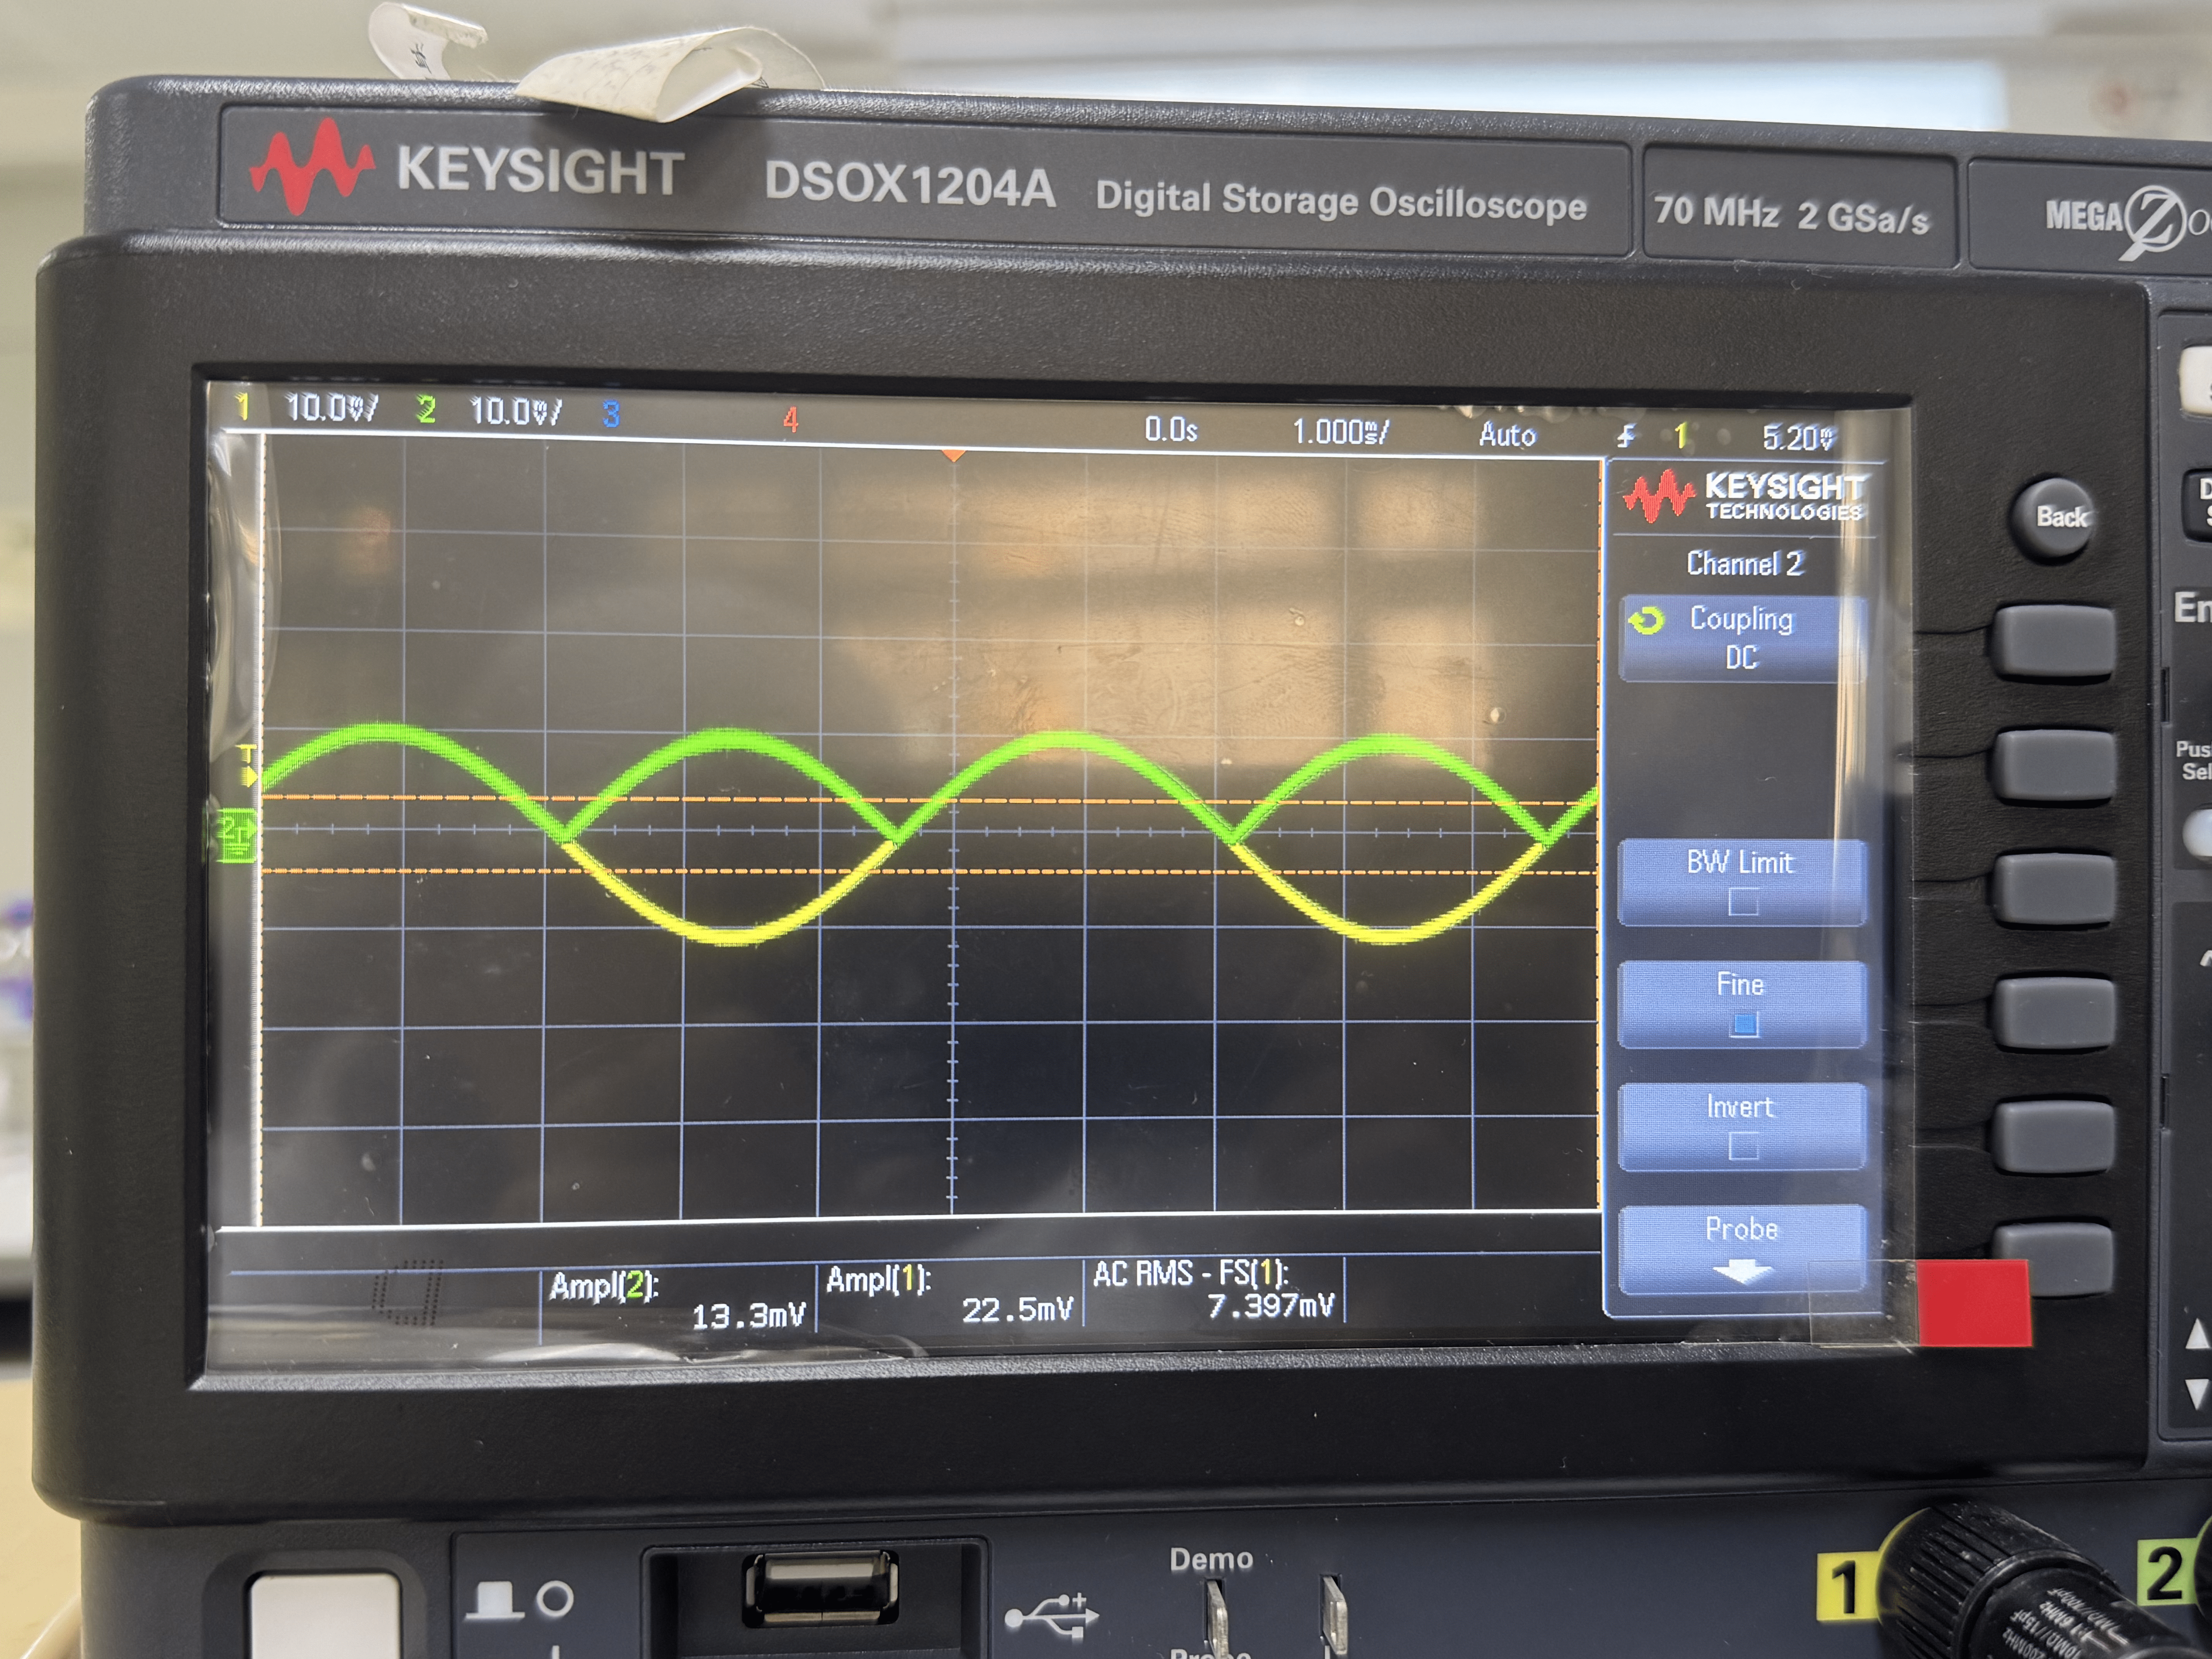
\includegraphics[width=0.5\linewidth]{Lab14/Images/lab14_0-1v.png}
            \caption{$V_i=0.1V$}
            \label{l14vi01v}
        \end{figure}
        \FloatBarrier
        \begin{figure}[h]
            \centering
            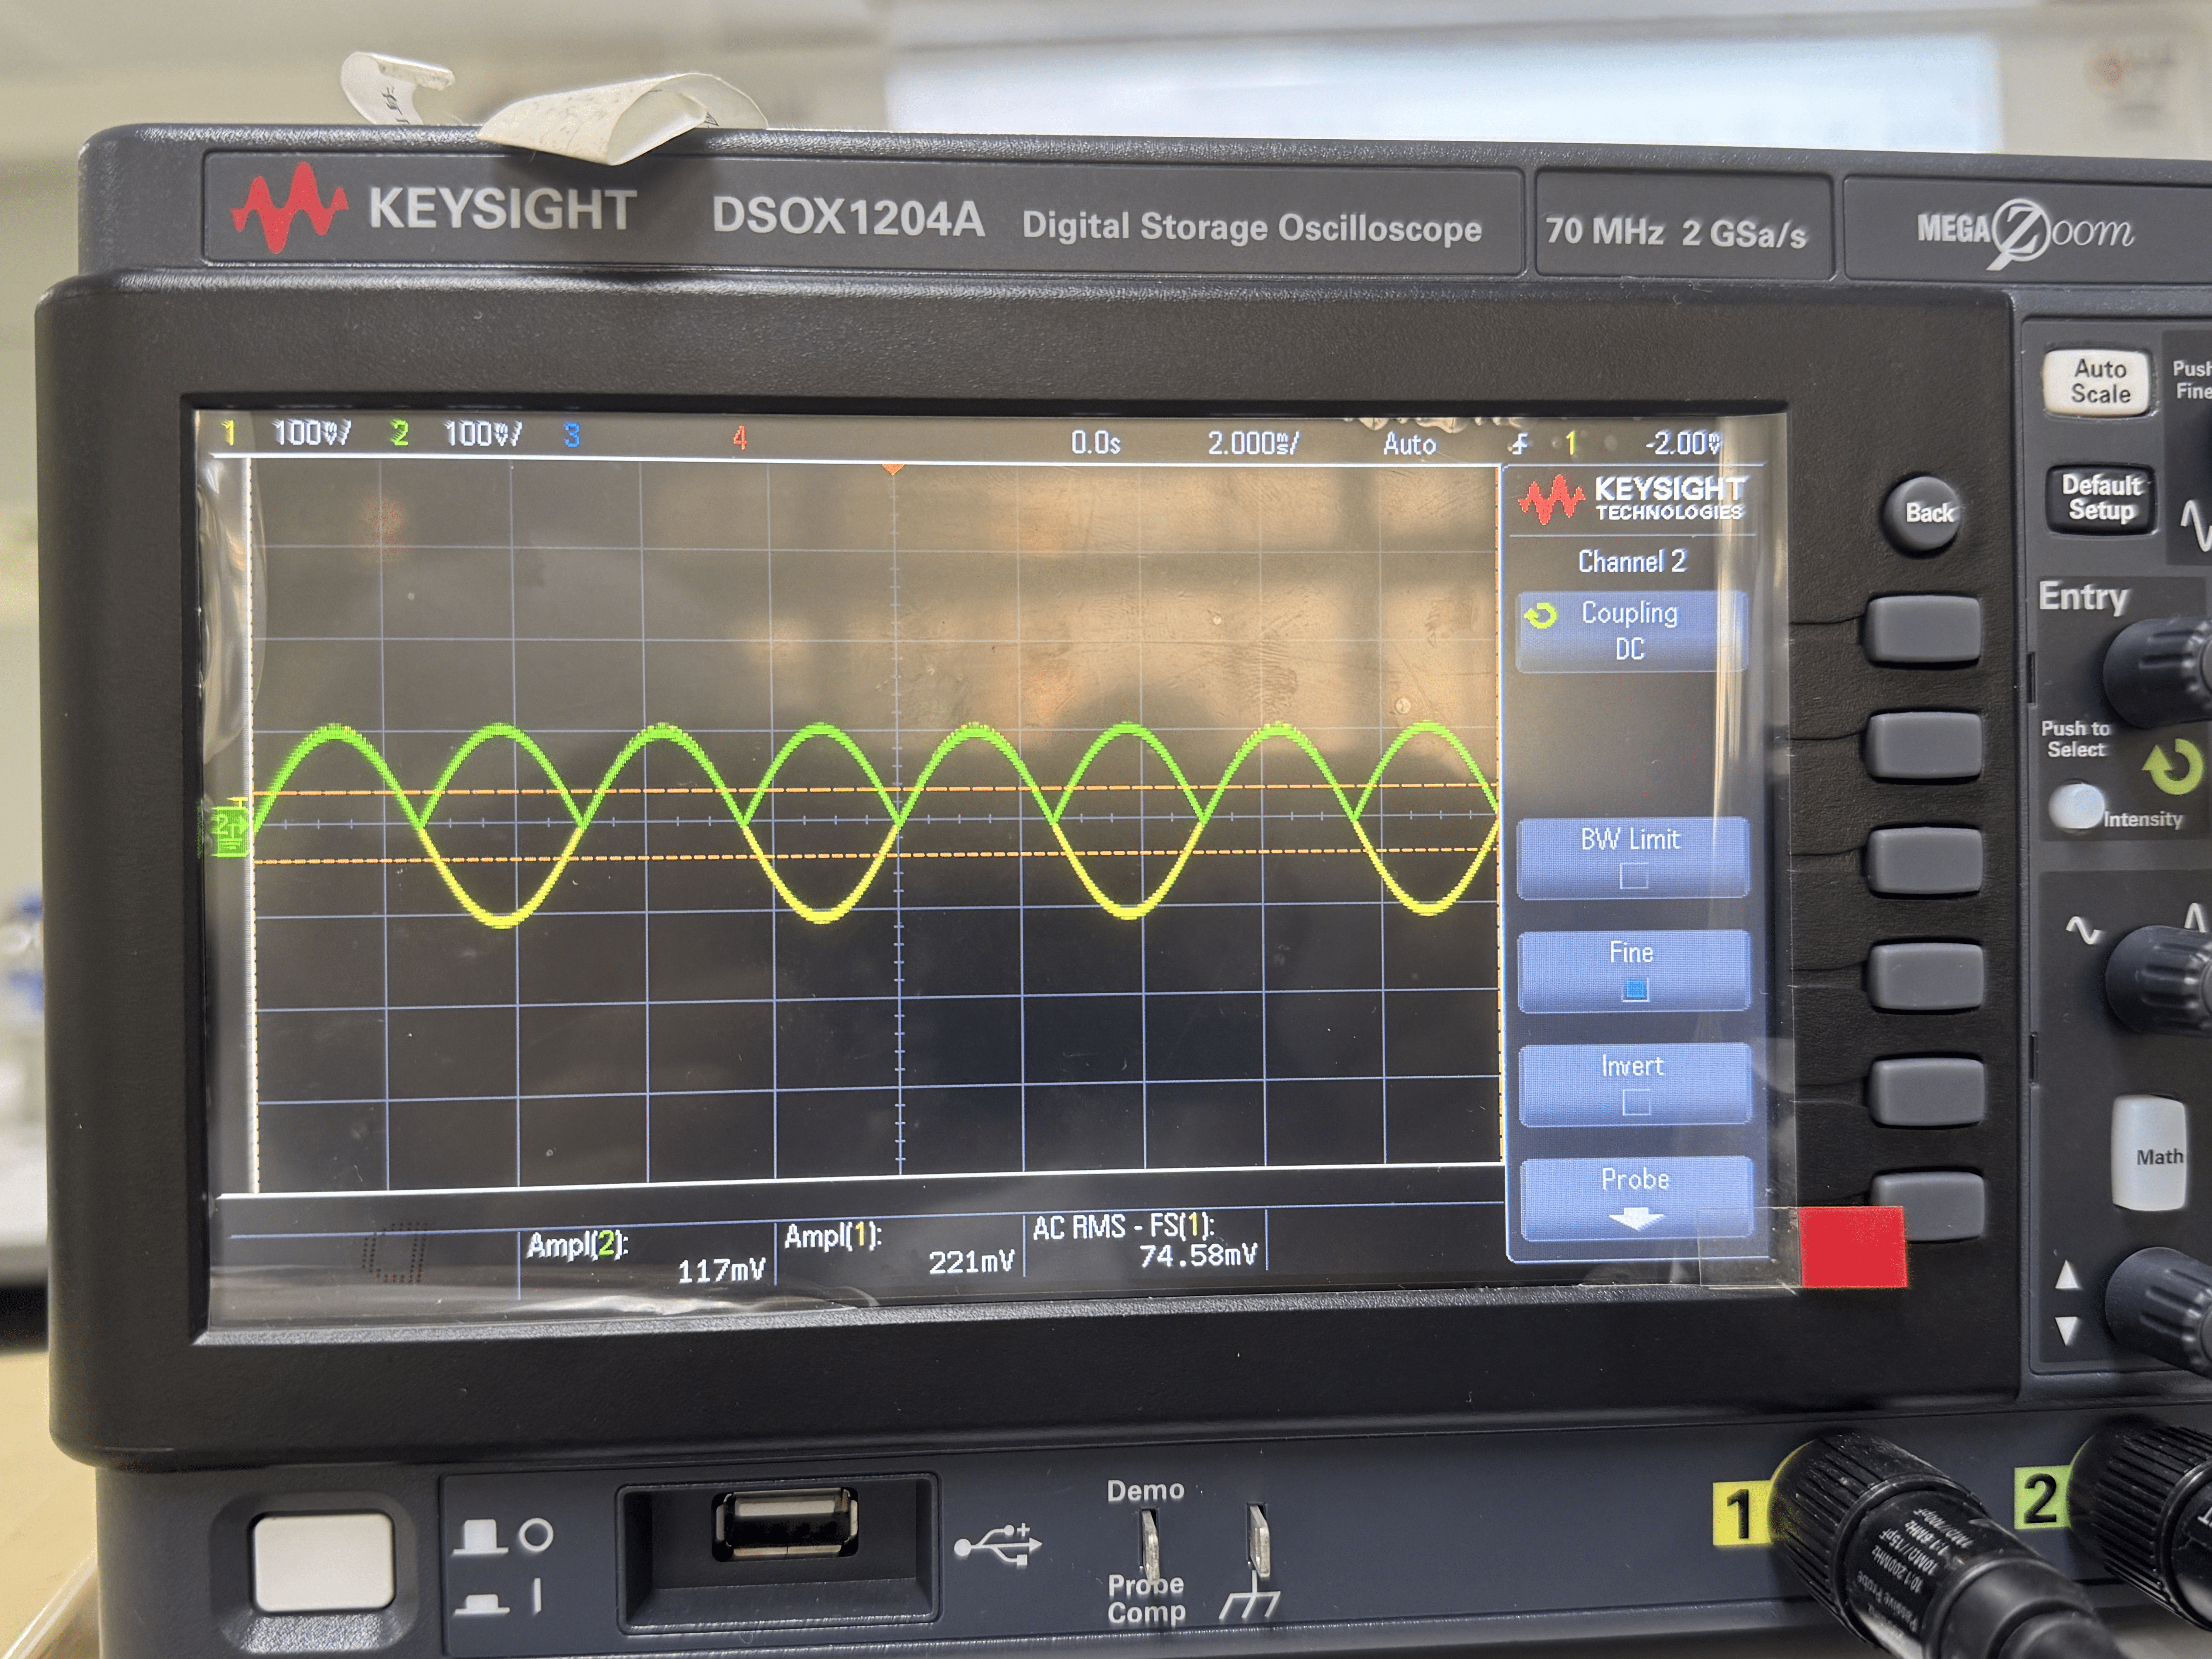
\includegraphics[width=0.5\linewidth]{Lab14/Images/lab14_1v.png}
            \caption{$V_i=1V$}
            \label{l14vi1v}
        \end{figure}
        \FloatBarrier
        \begin{figure}[h]
            \centering
            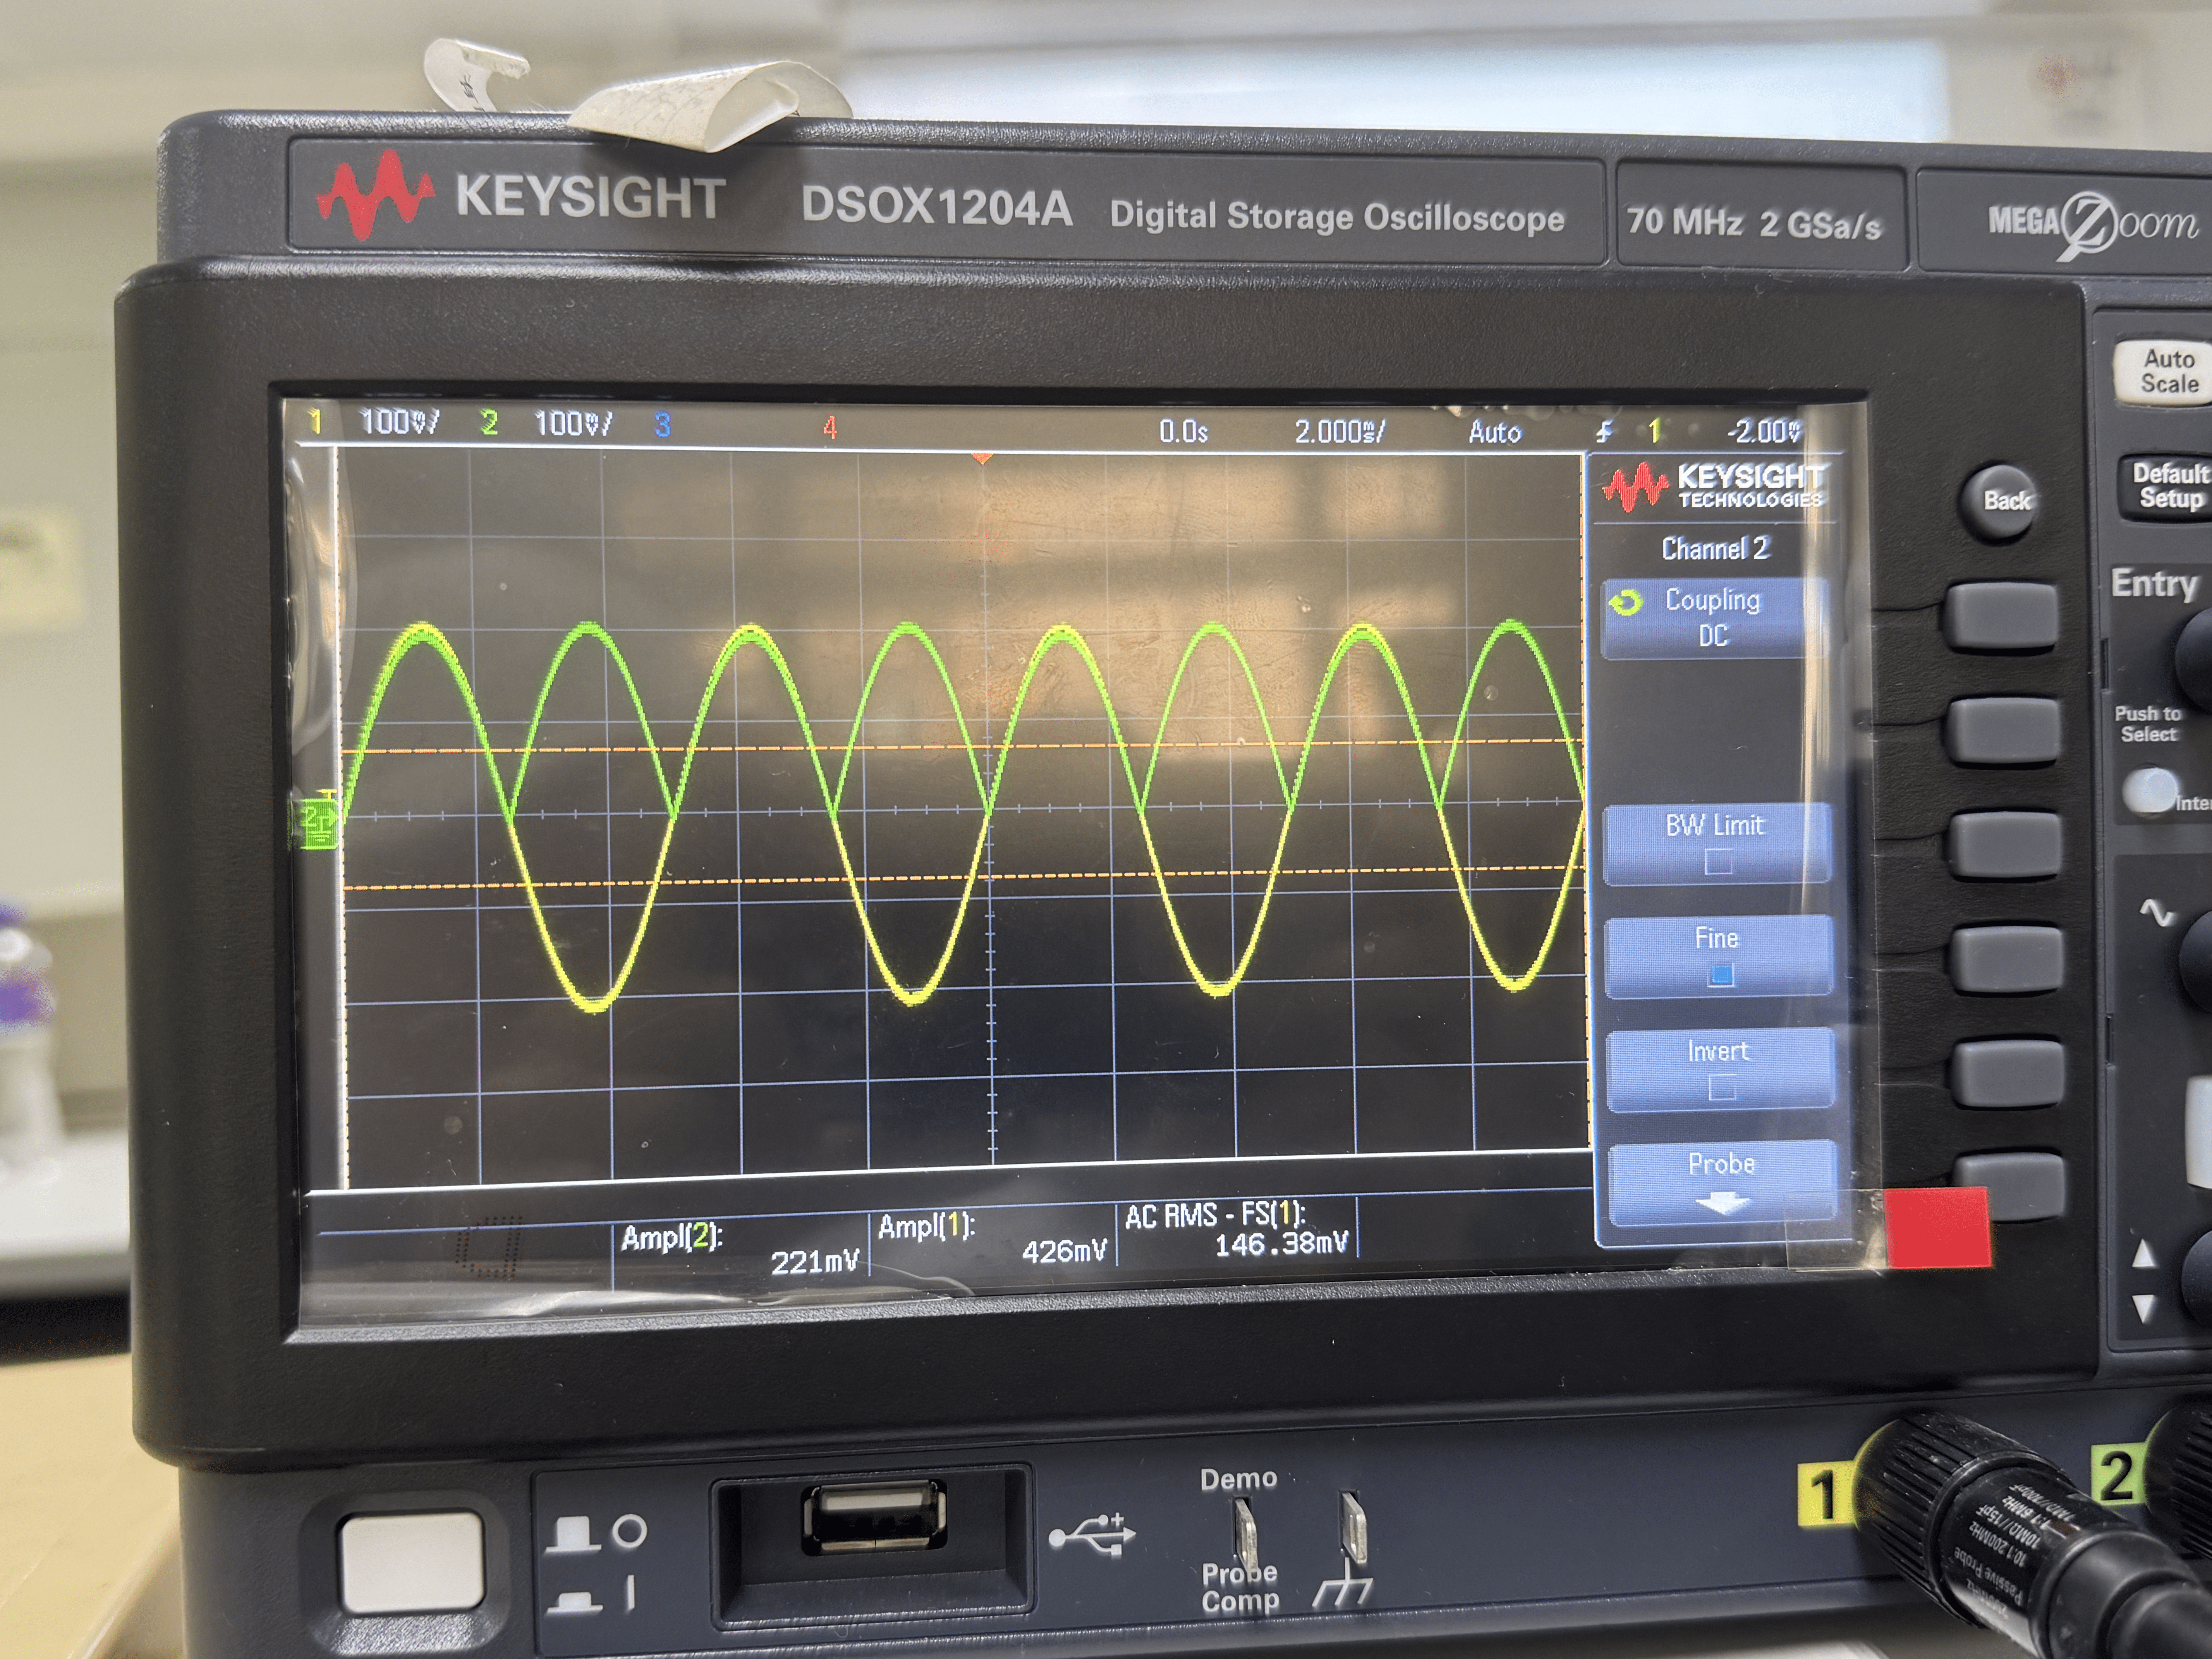
\includegraphics[width=0.5\linewidth]{Lab14/Images/lab14_2v.png}
            \caption{$V_i=2V$}
            \label{l14vi2v}
        \end{figure}
        \FloatBarrier
        \begin{figure}[h]
            \centering
            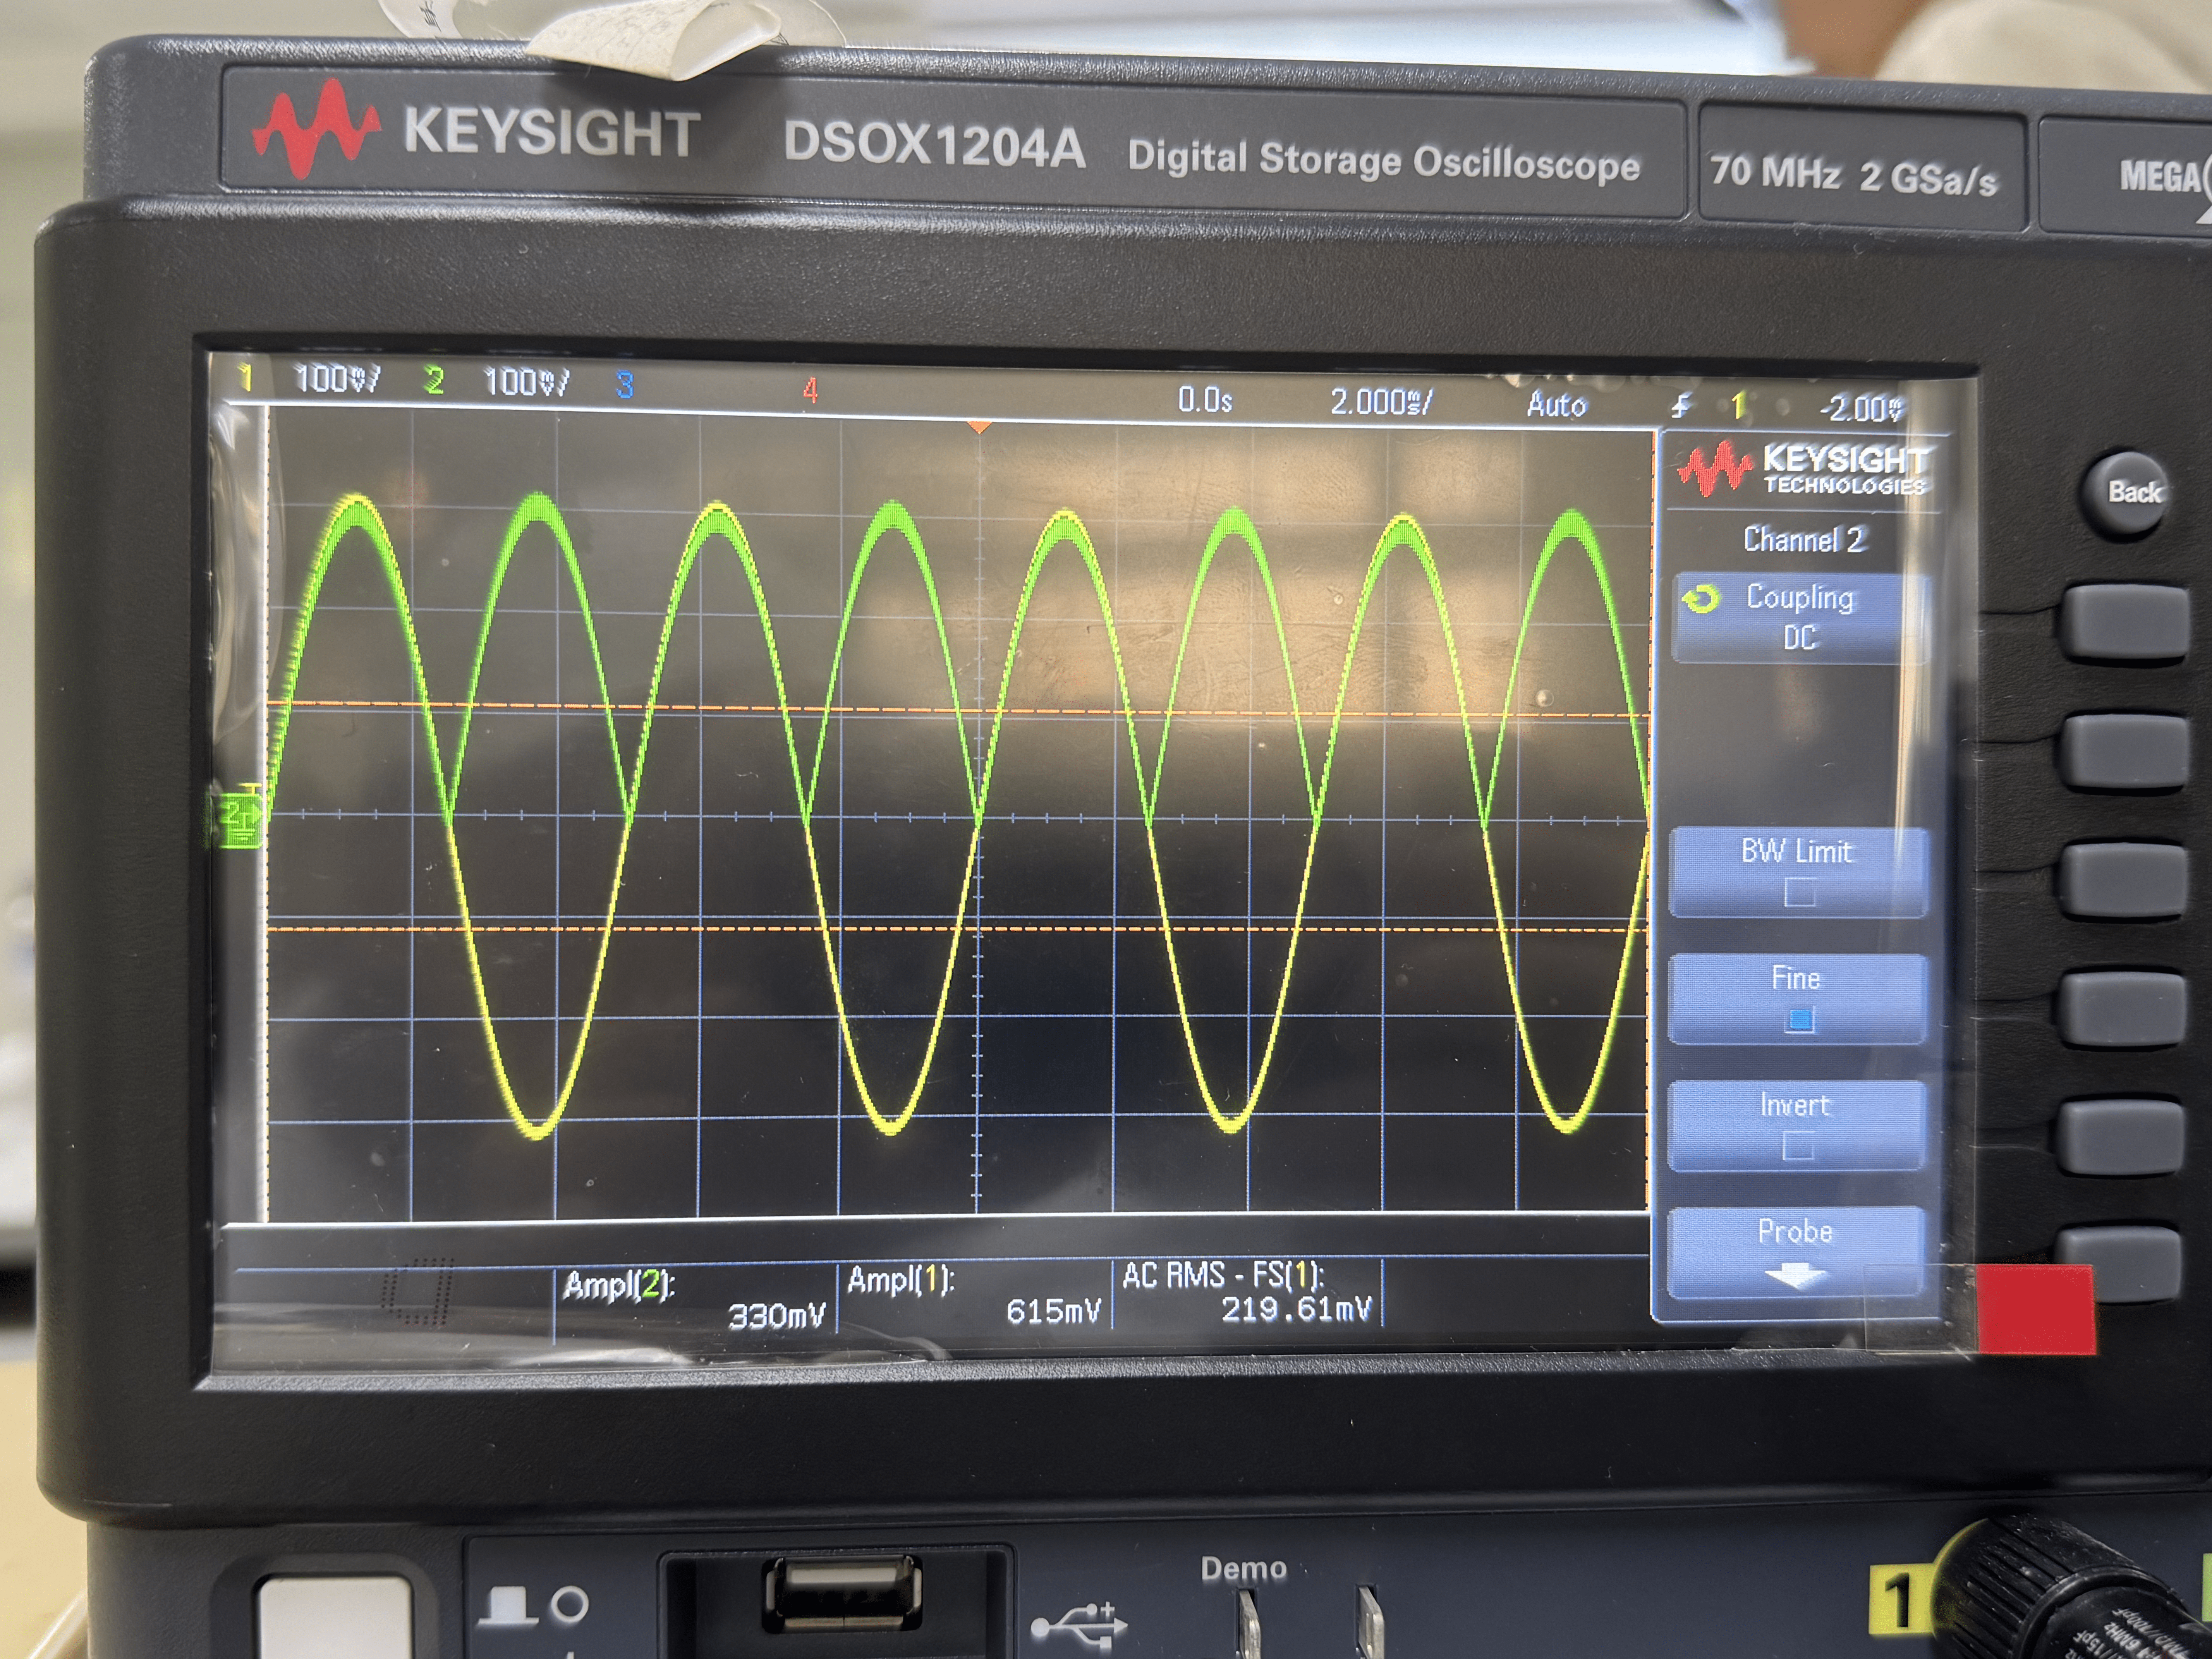
\includegraphics[width=0.5\linewidth]{Lab14/Images/lab14_3v.png}
            \caption{$V_i=3V$}
            \label{l14vi3v}
        \end{figure}
        \FloatBarrier
        \begin{figure}[h]
            \centering
            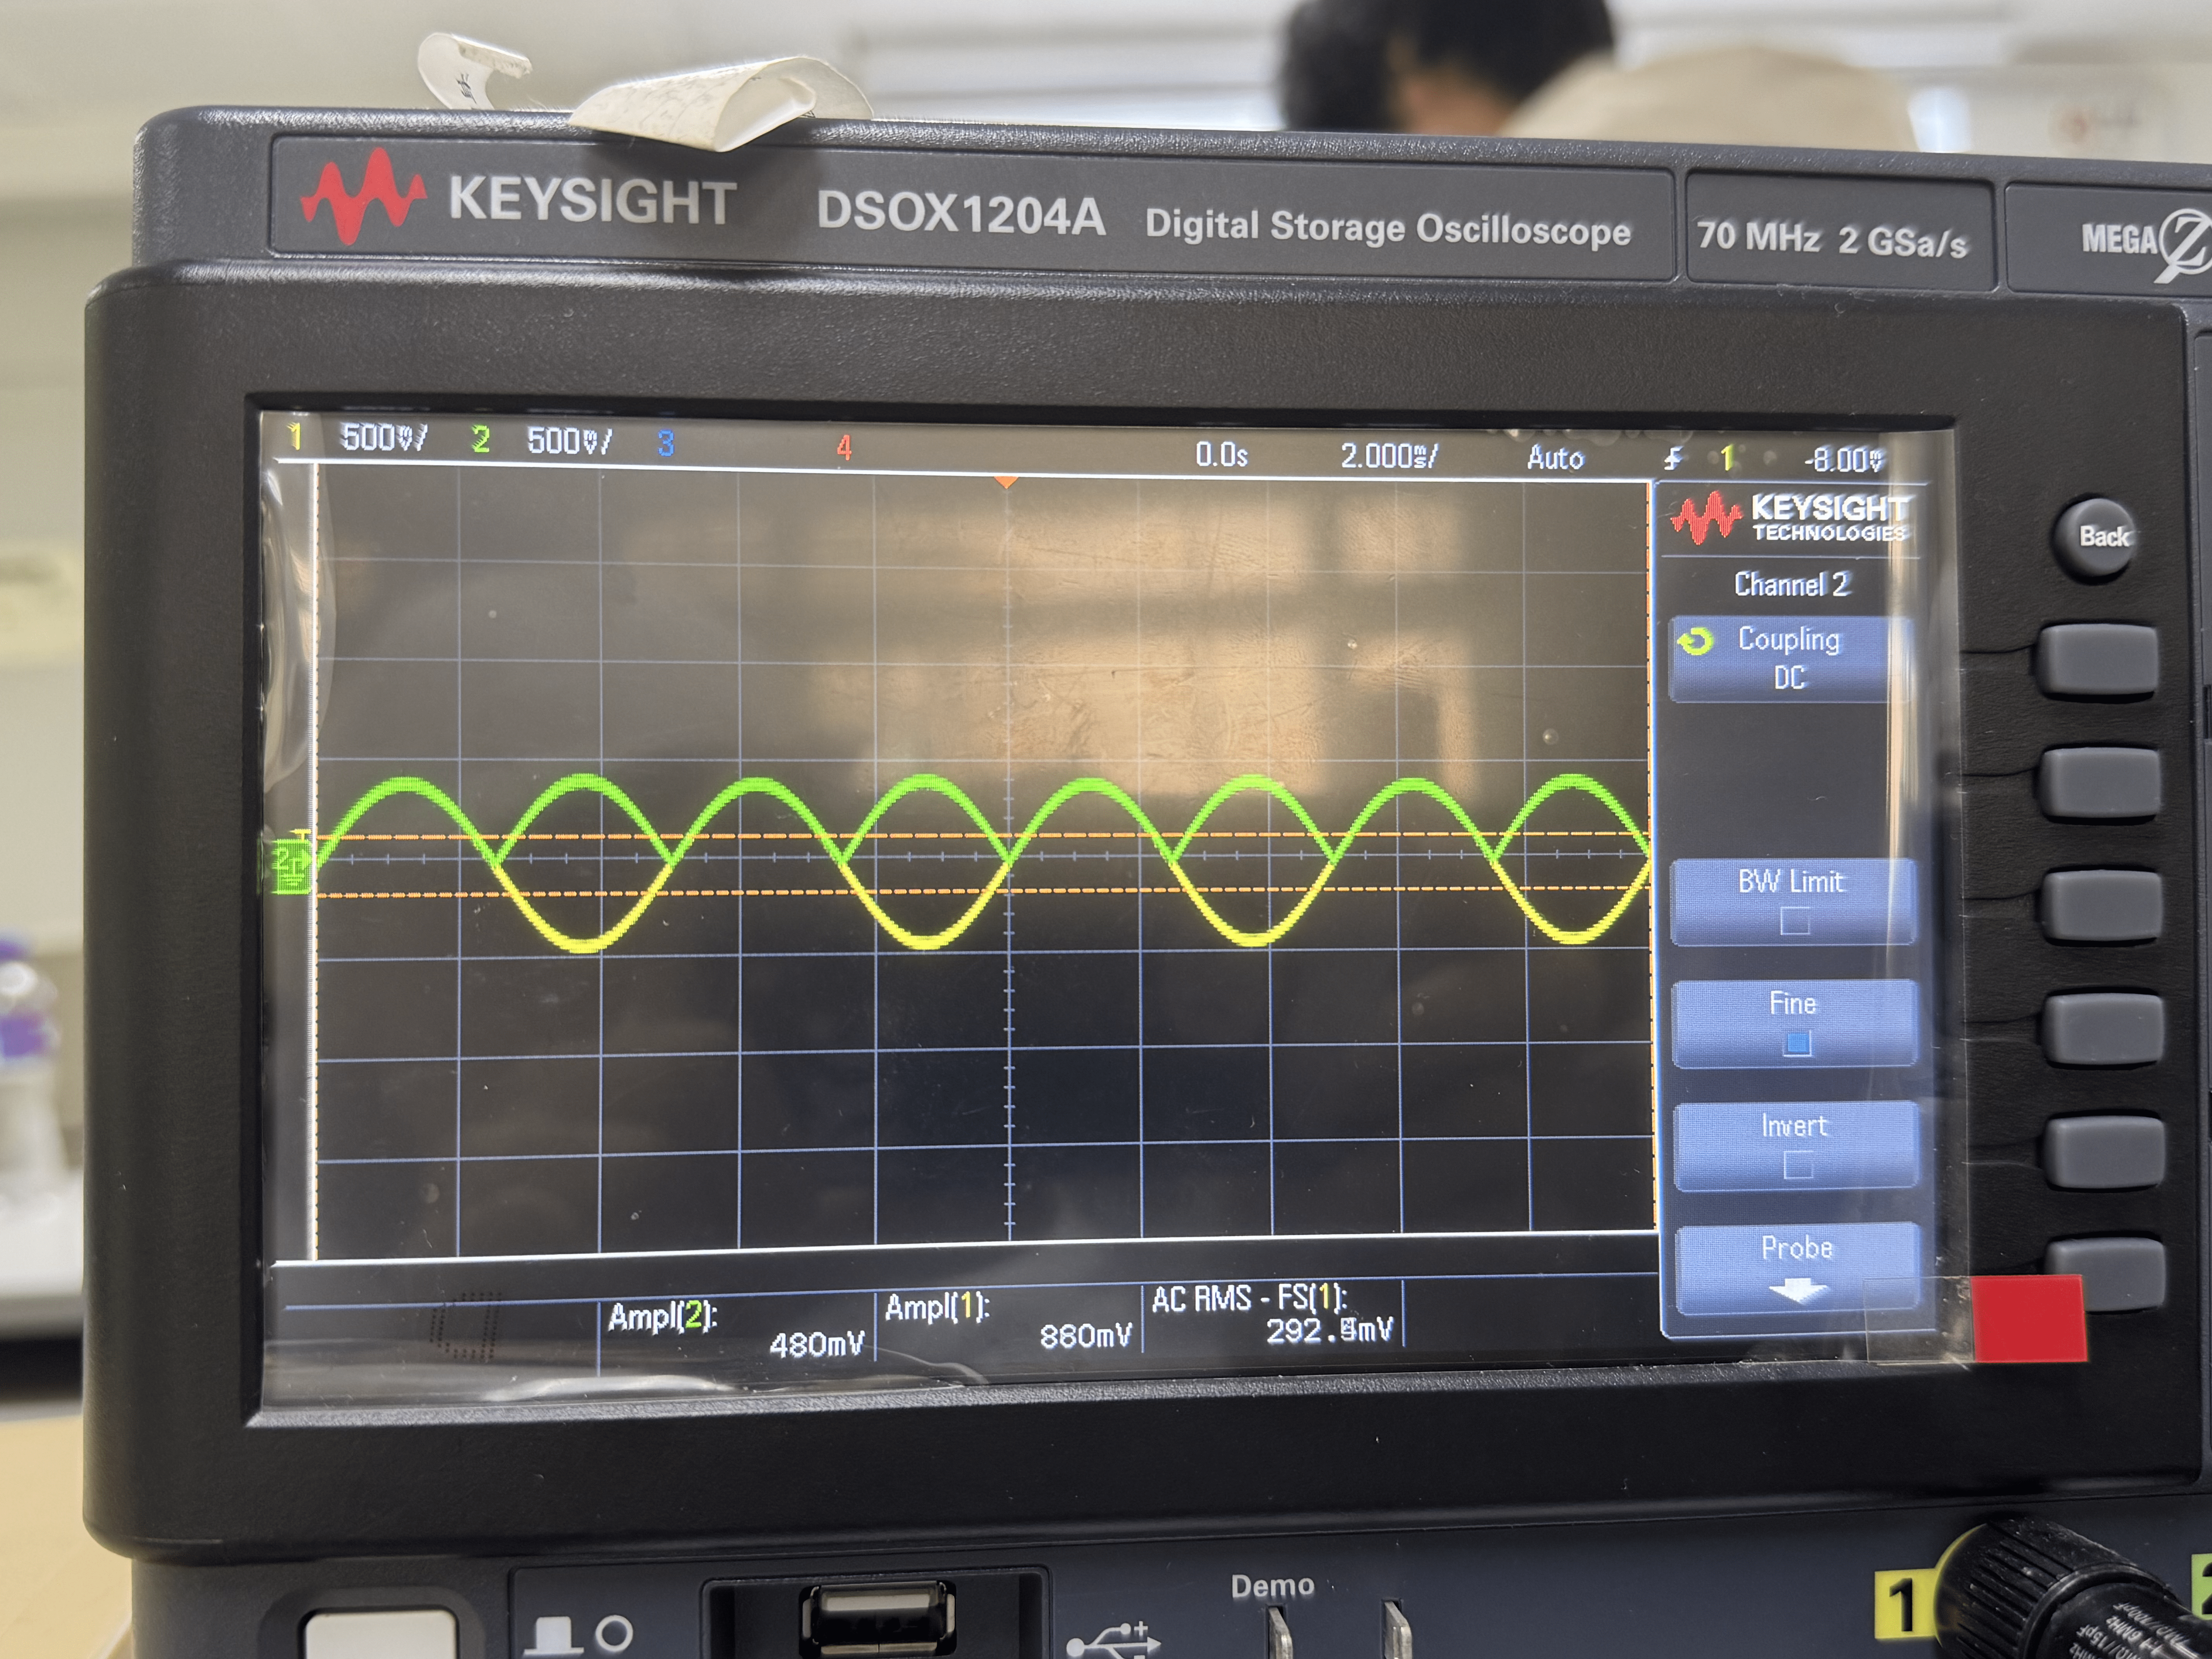
\includegraphics[width=0.5\linewidth]{Lab14/Images/lab14_4v.png}
            \caption{$V_i=4V$}
            \label{l14vi4v}
        \end{figure}
        \FloatBarrier
        \begin{figure}[h]
            \centering
            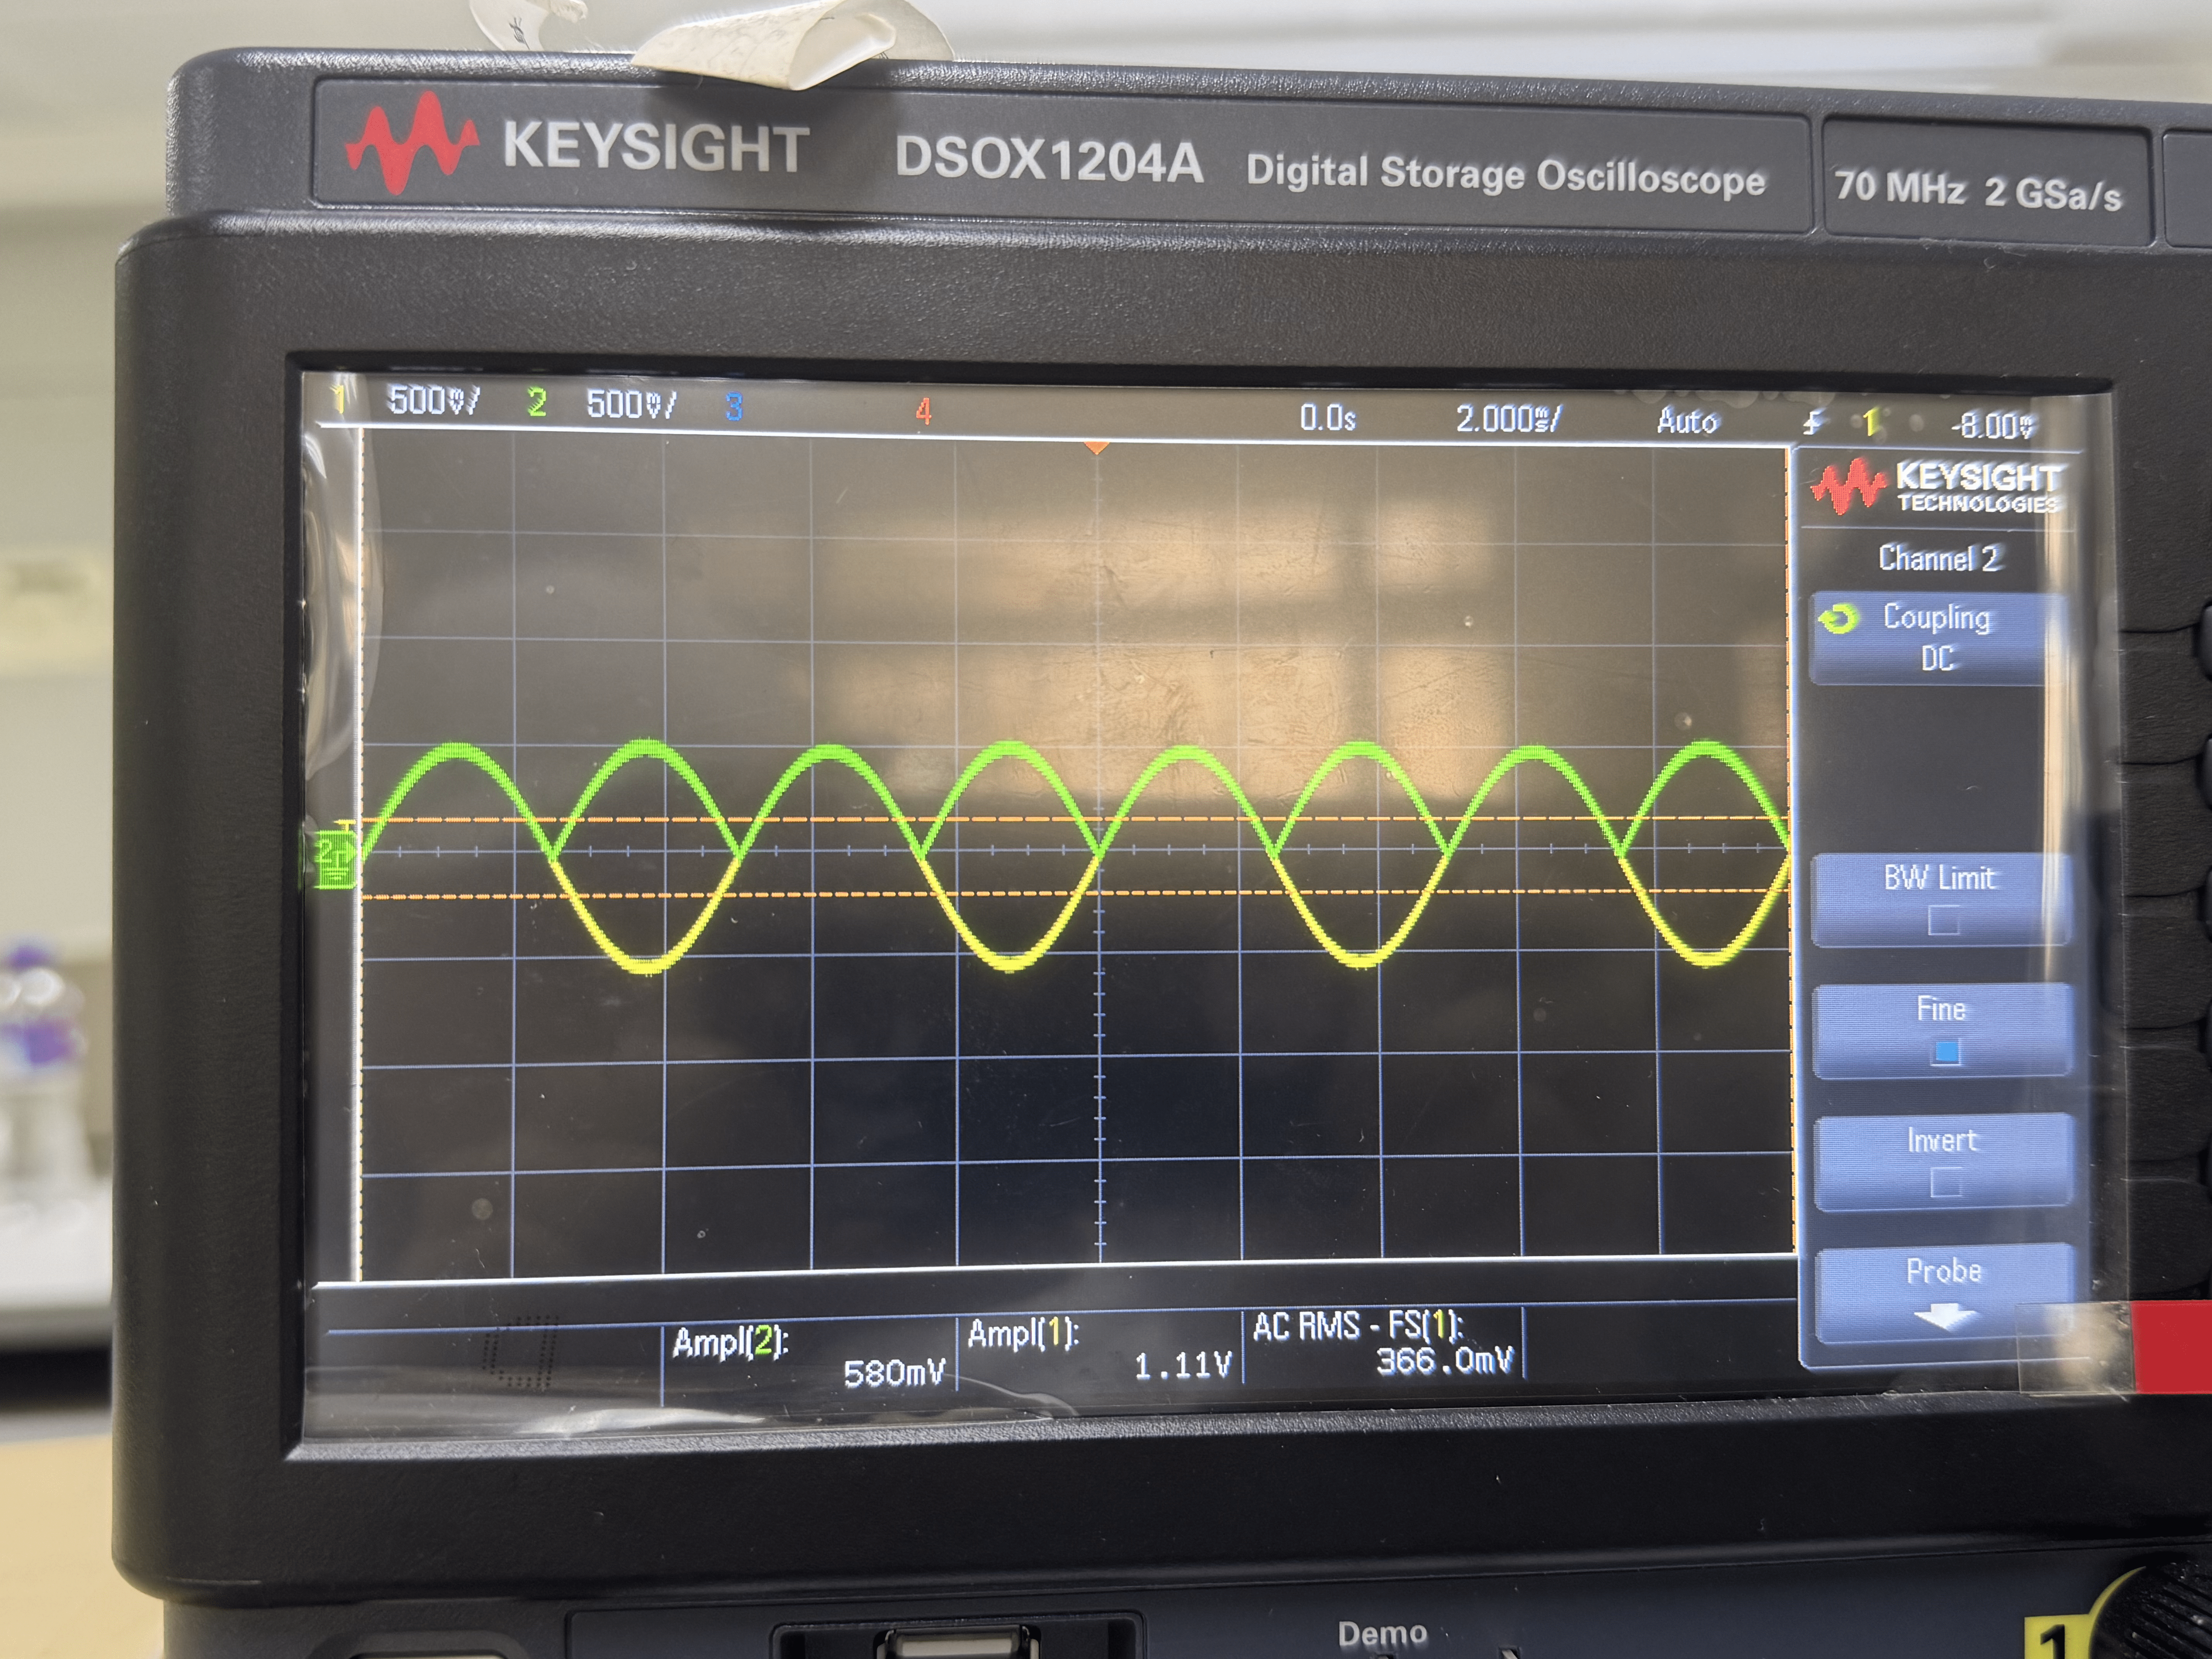
\includegraphics[width=0.5\linewidth]{Lab14/Images/lab14_5v.png}
            \caption{$V_i=5V$}
            \label{l14vi5v}
        \end{figure}
        \FloatBarrier
    From the figures above we can tell that all the negative signals are flipped into positive signals.\par
    And also the amplitude of the input and the output signals are smaller than threshold voltage of the diodes.\par
    \subsubsection{DC}
    Let $V_i$ be a DC voltage signal, and measure the data with digital multi-meter.\\
        \begin{table}[h]
        \centering
            \begin{tabular}{|c|c|c|c|c|c|c|}
            \hline
            $V_i$ & -12    & -5    & -1   & 1     & 5      & 12     \\ \hline
            $V_1$ & -0.408 & 0     & 0    & 0     & 0      & 1.562  \\ \hline
            $V_2$ & 8.68   & 3.799 & 1.03 & -1.42 & -5.504 & -9.4   \\ \hline
            $V_3$ & 2.548  & 1.64  & 0.32 & -1    & -5     & -8.875 \\ \hline
            $V_4$ & 8.195  & 3.353 & 0.66 & 0     & 0      & 1.549  \\ \hline
            $V_5$ & 5.617  & 3.353 & 0.66 & 0     & 0      & 0.0585 \\ \hline
            $V_o$ & 8.61   & 4.983 & 0.99 & 0.959 & 4.795  & 8.6    \\ \hline
        \end{tabular}
        \end{table}
        \FloatBarrier
    When $V_i$ are taking $\pm$12, the most of measured values are not equal to the theoretical relationships. It is because when the $V_i$ are taking that values, the condition of Equation.\ref{l14ceq1}, Equation.\ref{l14ceq2}, and virtual short is no longer satisfied.
    
\section{Discussion}
    When we are calculating the theoretical values of the circuit related to Op.Amp., we need to consider the condition of virtual short, which is affected by $V_i$ in this case.

\section{Conclusion}
    In conclusion, these two chapters strengthen my knowledge about Op.Amp. and full-wave rectifier, including practical usage and condition of use.